\documentclass[11pt, oneside]{book}
\usepackage[utf8]{inputenc}
\usepackage{graphicx}
\usepackage{hyperref}

\usepackage{times}
\usepackage{latexsym}
\renewcommand{\UrlFont}{\ttfamily\small}
\usepackage{graphicx}
\usepackage{adjustbox}

\usepackage{balance}
%% Useful packages
\usepackage{graphicx}
\usepackage{amsmath}
\usepackage{subcaption}
%\usepackage[table,xcdraw]{xcolor}
\usepackage{hyperref}
\usepackage{array}
\usepackage[title]{appendix}
\usepackage{adjustbox}
\usepackage{multirow}
\usepackage{arydshln}
%\usepackage{array}
\usepackage{booktabs}
\usepackage{flushend}
\usepackage{enumitem}
\usepackage{tabularx}
\usepackage{natbib}
\usepackage{xcolor}
\usepackage{amssymb}
\setcitestyle{numbers,open={[},close={]},comma}
\setcounter{secnumdepth}{3} 
\newcommand{\paragraphHd}[1] {\vspace{3pt}\noindent\textbf{#1}}

\newcommand{\method}[1]{HAM$_{\text{\,#1}}$}
\newcommand{\charm}[1]{CHARM$_{\text{\,#1}}$}
\newcommand{\wiki}[1]{Wiki-#1}
\newcommand{\attribute}[1]{\textbf{\emph{#1}}}
\newcommand{\paragraphHdTop}[1] {\noindent\textbf{#1}} % use for first in a series of paragraphHd's
\newcommand{\paragraphHd}[1] {\vspace{3pt}\noindent\textbf{#1}}

\newcommand{\squishlist}{
 \begin{list}{$\bullet$}
  { \setlength{\itemsep}{0pt}
     \setlength{\parsep}{1pt}
     \setlength{\topsep}{1pt}
     \setlength{\partopsep}{0pt}
     \setlength{\leftmargin}{1.5em}
     \setlength{\labelwidth}{1em}
     \setlength{\labelsep}{0.5em} } }

\newcommand{\squishend}{
  \end{list}  }
  
  
\newcommand{\sig}[1]{#1*}
\newcommand{\nsig}[1]{#1\phantom{*}}
\newcommand{\bsig}[1]{\textbf{#1}*}
\newcommand{\bnsig}[1]{\textbf{#1}\phantom{*}}
\newcommand{\best}[1]{\textbf{#1}}

\hyphenation{lib-ra-ry}

\usepackage{comment}

\begin{document}

\chapter[CHARM]{Conversational Hidden Attribute Retrieval Model 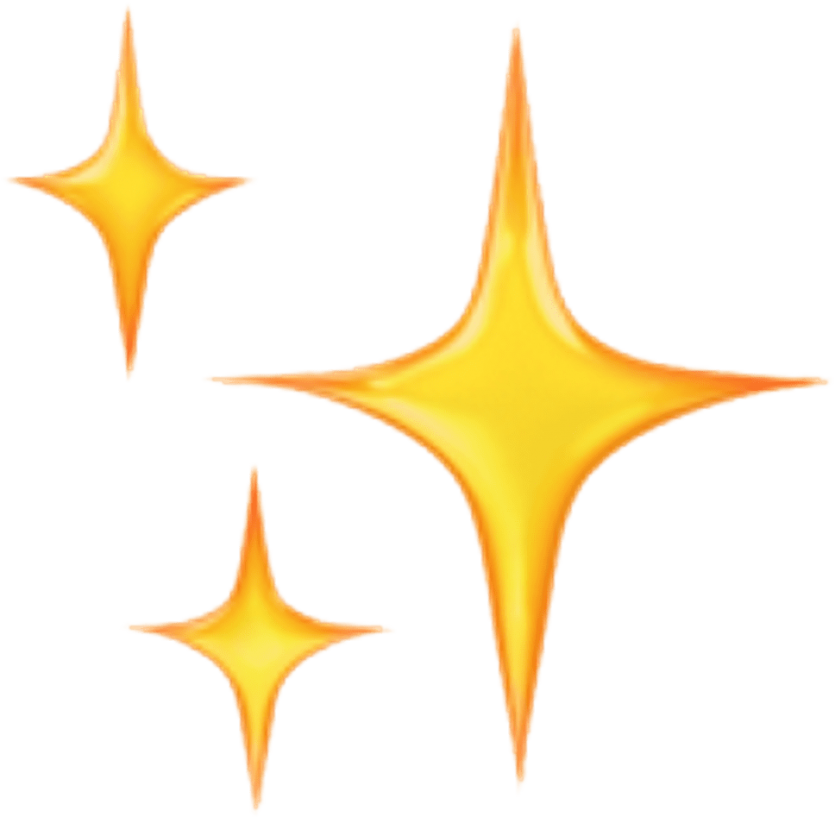
\includegraphics[scale=0.03]{stars.png}}

\section*{Abstract}
\label{abstract}

%\ \\%[0.25cm]

\droppedcapital{P}{ersonal} knowledge is a versatile resource that is valuable for a wide range of downstream applications.
Background facts about users can allow chatbot assistants to produce more topical and empathic replies.
In the context of recommendation and retrieval models, personal facts can be used to customize the ranking results for individual users.

A \textit{Personal Knowledge Base}, populated with personal facts, such as demographic information, interests and interpersonal relationships, is a unique endpoint for storing and querying personal knowledge. 
Such knowledge bases are easily interpretable and can provide users with full control over their own personal knowledge, including revising stored facts and managing access by downstream services for personalization purposes.

To alleviate users from extensive manual effort to build such personal knowledge base, we can leverage automated extraction methods applied to the textual content of the users, such as dialogue transcripts or social media posts. Conventional extraction methods specialize on well-structured data, such as biographical texts or encyclopedic articles, which are rare for most people.
In turn, conversational data is abundant but is challenging to process and requires specialized methods for extraction of personal facts.

In our research we address the acquisition of personal knowledge from conversational data. We propose several novel deep learning models for inferring speakers' personal attributes:
\begin{itemize}
    \item Demographic attributes, \textit{age}, \textit{gender}, \textit{profession} and \textit{family status} are inferred by \textbf{HAMs} - hierarchical neural classifiers, based on attention mechanism. HAMs efficiently transfer learn between different types of conversational data and provide interpretable predictions.
    
    \item Long-tailed personal attributes, \textit{hobby} and \textit{profession}, are predicted with \textbf{CHARM} - a zero-shot learning model, overcoming the lack of labeled training samples for rare attribute values. By linking conversational utterances to external sources PRIDE is able to predict attribute values, which it never saw during training.
    
    \item \textit{Interpersonal relationships} are inferred with \textbf{PRIDE} - a hierarchical transformer-based model. To accurately predict fine-grained relationships, PRIDE leverages personal traits of the speakers and the style of conversational utterances.
\end{itemize}

Experiments with various conversational texts, including Reddit discussions and movie scripts, demonstrate the viability of our methods and their superior performance compared to state-of-the-art baselines.

\section{Introduction}

\paragraphHd{Motivation\textnormal{:}}
While interest in dialogue agents has grown rapidly in recent years, creating agents capable of holding personalized conversations remains a challenge. 
The knowledge of the user's demographic attributes, such as \textit{age} or \textit{family status}, is a crucial step towards a user-friendly dialogue system, capable of adjusting its speech style and offering relevant suggestions with respect to the user's traits.

For meaningful and diverse dialogues with a real person, a system should be able to infer knowledge about the person's background from her utterances. 
Consider the following example, where $H$ stands for a human and $A$ for a dialogue agent:\vspace{0.1cm}\\
%\textcolor{red}{example of conversation with an agent}
\hspace*{0.3cm}{H:} {\em What's the best place for having brekky?}\\
\hspace*{0.3cm}{A:} {\em The porridge at Bread and Cocoa is great.}\\
%\hspace*{0.3cm}{H:} {\em Any suggestions for the four of us later?} \\
\www{
\hspace*{0.3cm}{H:} {\em Any suggestions for us and the kids later? We already visited the zoo.} 
}\\
%\hspace*{0.3cm}\phantom{H:} {\em We already visited the zoo.}\\
%\hspace*{0.3cm}{A:} {\em There's an interesting museum on war history nearby.}
\www{
\hspace*{0.3cm}{A:} {\em There's the San Francisco Dungeon, an amusement ride with scary city history.}\\
%\hspace*{0.3cm}\phantom{H:} {\em an amusement ride with scary city history.}
}
\vspace{0.05cm}

\noindent From the word `brekky' in the first $H$ utterance, 
the system understands that the user is Australian
and may thus like porridge for breakfast. 
However, the 
%implicit 
cue is missed that the user 
{is with pre-teen children (talking about kids and the zoo)},
and the resulting suggestion is inappropriate for young children. 
Instead, with awareness of this knowledge, a better reply could have been:\vspace{0.1cm}\\
\hspace*{0.3cm}{A:} {\em I bet the kids loved the sea lions, so you should also see the dolphins at Aquarium of the Bay}
\vspace{0.1cm}

\noindent A possible remedy to improve this situation is to include user information
into an end-to-end learning system for the dialogue agent. 
However, any user information would be bound to latent representations rather than explicit attributes.
Instead, we propose to capture such attributes explicitly and add them to a personal knowledge base, which will then be a distant source of background knowledge
for personalization in downstream applications such as
Web-based chatbots and agents in online forums.

To populate the PKB without the user's manual supervision, we need to leverage the methods for automatic personal information extraction. There has been ample work on information extraction from structured external sources, such as Wikipedia entries or news stories. However, there is little hope of finding the personal information about each individual user in encyclopedic articles. 

Instead, personal facts can be extracted from unstructured textual sources, such as user's conversational data. Such data, in form of dialogue transcriptions or social media posts, is abundant and rich in signals about the given user's persona. However, conventional methods for information extraction from well-comprehensible text genres fail to perform properly given conversations as input. Dialogue utterances are short, noisy and colloquial, which necessitates creating novel extraction methods, tailored specifically to conversational data.

This work addresses these issues by proposing methods to \textit{infer} personal facts from dialogues based on implicit cues. The proposed approach takes advantage of the hierarchical dialogue structure to outperform previous information extraction models.

\paragraphHd{State of the Art and its Limitations\textnormal{:}}
Currently the most successful dialogue agents are task-oriented, 
for instance, supporting users with car navigation or delivery orders
(e.g., \cite{dial6,AAAI1816104}).
This makes the task considerably easier, because the system has to focus on specific words, related to the topic. We, in contrast, strive to be able to extract information for domain-independent dialogue, from everyday conversation, where the relevant facts are only latent.
General-purpose chatbot agents show decent performance in
benchmarks (e.g., \cite{bot1,pers1,dial8}), 
but critically rely on sufficient training data and
tend to lack robustness when users behave in highly varying ways.
Very few approaches have considered incorporating explicit knowledge
on individual users, and these approaches have assumed that personal attributes
are explicitly mentioned in the text \cite{dial7,zhang2018personalizing,jing-kambhatla-roukos:2007:ACLMain}.

To illustrate that identifying explicit mentions of attributes is insufficient,
we developed an oracle to obtain an upper bound on the performance of pattern-based approaches, such as \cite{dial7}. This oracle, which is described in Section \ref{sec:baselines}, assumes that we have perfect pattern matching that correctly extracts an attribute value every time it is mentioned.
(When multiple attribute values are mentioned, we assume the oracle picks the correct one.)
This oracle routinely performs substantially worse than our proposed methods, demonstrating that extracting information from utterances requires inferring the presence of attribute values that are never explicitly stated.

\www{
On the other hand, many efforts have considered the problem of profiling social media users in order to predict latent attributes such as \textit{age}, \textit{gender}, or \textit{regional origin} (e.g., \cite{Rao:2010,burger:EMNLP11,Schwartz2013PersonalityGA,sap:EMNLP14,flekova:ACL16:long,kim:ACL17:short,vijayaraghavan:ACL17:short,bayot:MOD17,fabian2015privacy}). While social media posts and utterances are similar in that both are informal, the former can be associated with many non-textual features that are unavailable outside of the social media domain 
(e.g., social-network friends, likes, etc. and explicit self-portraits of users).
We consider several user profiling baselines that rely on only textual features and find that they do not perform well on our task of inferring attributes from 
conversational utterances.
}

\paragraphHd{Approach and Contributions\textnormal{:}}
We devise a neural architecture, called \textbf{H}idden \textbf{A}ttribute \textbf{M}odels (HAMs) \cite{tigunova:ham:2019}, 
trained with
subject-predicate-object triples to predict objects on a per-predicate basis,
e.g., for a subject's \textit{profession} or \textit{family status}.
The underlying neural network learns to predict a scoring
of different objects (e.g., different professions) for
a given subject-predicate pair
by using attention within and across utterances to infer object values.
For example, as illustrated later in Table \ref{tab6}, our approach infers that a subject
who often uses terms like `\textit{theory}', `\textit{mathematical}', and `\textit{species}' is likely to be a \textit{scientist}, while a subject who uses terms like `\textit{senate}', `\textit{reporters}', and `\textit{president}' may be a \textit{politician}.


The salient contributions of this work are the following: 
\begin{itemize}
\item a viable method for learning personal attributes from
conversations, based on neural networks with novel ways of
leveraging attention mechanisms and embeddings,
\item an extensive experimental evaluation of various methods on
Reddit, movie script dialogues, and crowdsourced personalized conversations (PersonaChat),
\item \www{
an experimental evaluation of the transfer learning approach: 
%the applicability of 
leveraging
%the vast amount of
ample data from
user-generated social media texts (Reddit) for inferring users' latent attributes from data-scarce speech-based dialogues (movie scripts and PersonaChat).
}
\end{itemize}



\section{Related work}

In this section we discuss related work concerning the methods that are used in HAMs. First, we give an overview of the application of neural models utilizing attention mechanism, which is the main building block in our best performing models. Second, we describe the methods for building hierarchical representations of the conversational data. We also refer the reader to Section \ref{back_rel} for a comprehensive overview of the author profiling methods.

\subsection{Neural Models with Attention} 

The role of attention weights has been studied for various neural models, including feed-forward networks \cite{vaswani2017attention}, CNNs, \cite{atten4} and RNNs \cite{bahdanau2014neural}. Recently, neural models enhanced with attention mechanisms have boosted
the results on various NLP tasks \cite{atten1,atten9,atten2}, particularly 
in conversational domain for response generation \cite{atten7, zhang2019recosa}
or spoken language understanding \cite{Chen2016}. 

In response generation task, attention is used to align the context and target utterance representation \cite{atten7}. \citet{zhang2019recosa} extends it with additional self-attention layers for both context and response representations. \citet{Chen2016} uses attention to estimate the relevance of the previous knowledge stored in memory to the input utterances; the response is produced using the attention distribution, calculated by matching each input utterance to the memory vectors.

Transformer \cite{vaswani2017attention} is a state-of-the-art sequence-to-sequence deep learning model based on self-attention mechanism. Transformer is used across various NLP tasks, both as a standalone model and as a part of other neural architectures. In particular, in conversation domain Transformer has been used to produce utterance representations \cite{li2020hierarchical, shan2020contextual}.

\subsection{Hierarchical conversational models} 
\label{ham_hier}

Hierarchical models to represent conversations were introduced in \citet{serban2016building}, which applied RNNs to hierarchically build the representations of utterances and the dialogue context, solving response generation task. \citet{atten8} also decoded conversational responses, introducing attention mechanism into the hierarchical encoder architecture. In \citet{atten8} the utterance and word representations are formed as the attention-weighted averages of the hidden states in word and utterance level RNNs. 

Hierarchical attention models are also utilized for other conversational NLP tasks, such as dialogue state tracking \cite{shan2020contextual} or emotion recognition in conversations \cite{li2020hierarchical, ma2021han}. A common approach is to create word representations with BERT and utterance representations with Transformer encoder \cite{shan2020contextual, li2020hierarchical} or RNN \cite{ma2021han}.

There is also ample research on applying hierarchical attention to speaker attribute prediction. \citet{lynn2020hierarchical} use attention mechanism with the word and utterance representations created by an RNN to predict personality traits of the Facebook users. The study \cite{li2019improving} exploits hierarchical model to predict \textit{age}, \textit{gender} and \textit{location} information of Weibo users.

Compared to most hierarchical models, the architecture of HAMs is more light\hyp{}weight, because it creates speaker representations with an attention mechanism directly, without additionally running an RNN or Transformer models on the attention-weighted words. Thus HAMs are less prone to overfitting and require less computational resources. Regardless of its simplicity, our proposed architecture can still make meaningful predictions in classification tasks with large number of classes, such as \textit{profession} prediction, as opposed to few possible classes in related studies \cite{lynn2020hierarchical, li2019improving}. 



 






\section{Background}
\label{background}

Interactions between people can have multiple fine-grained features, describing various aspects of their communication. For example, interactions can be characterized by attachment style (such as \textit{commitment} or \textit{avoidance}) \cite{qamar2021relationship} or power hierarchy (\textit{subordinate} or \textit{superior}) \cite{prabhakaran2014predicting}. There are ample related social studies researching these characteristics; yet, there is no formal ontology for them \cite{rashid2018characterizing}. One way to organize the features of interpersonal interactions was proposed by \cite{rashid2017dimensions}, defined as \textit{dimensions} of the relationships.

Most of the relationships that we defined for our experiments also have particular interpersonal characteristics. For example, the \textit{enemy} relationship can be described as \textit{competitive} as opposed to \textit{cooperative}; the relationship between \textit{parent} and \textit{child} is in most cases \textit{intimate}. Thus, we find it beneficial to enhance the relationship prediction model with the known features of the speakers' interactions. 

We use the definition of \textit{interpersonal dimensions} \cite{wish1976perceived} of speakers' interactions and relationships, following classification of \citet{rashid2018characterizing}, which we used as an additional input to our model. We note that the discussed interpersonal dimensions are descriptive of the relationship between a particular pair of speakers, but not of the relationship type in general (for example, the interaction between \textit{colleagues} can be both \textit{cooperative} and \textit{competitive}). However, in general any interpersonal dimension can be more or less typical for a relationship type; we use this information to give the model hints about applicable predictions.

\citet{rashid2018characterizing} consider 11 interpersonal dimensions, divided into dimensions of relationships and interactions, as shown in Table \ref{dimensions}. In our model we use all proposed dimensions to provide a comprehensive summary of the relationship's fine-grain characteristics. %For details on each dimension we refer the reader to the original paper \cite{rashid2018characterizing}.
\citet{rashid2018characterizing} also provide a conversational dataset, where every utterance has annotations for each considered interpersonal dimension. We utilize this dataset to pretrain a model for utterance-level dimension classification and create separate representations for each dimension, which are later used in PRIDE.

\begin{table}[t!]
\centering
\begin{adjustbox}{width=0.7\textwidth}
\begin{tabular}{@{}l|ll@{}}
\multirow{4}{*}{relationships} & cooperative vs. noncooperative & equal vs. hierarchical\\ 
 & pleasure vs. work oriented & intense vs. superficial \\ 
 & intimate vs.unintimate & active vs. passive \\ 
 & temporary vs. long term \\ \hline
\multirow{2}{*}{interactions}  & cooperative vs. noncooperative & active vs. passive \\ 
 & concurrent vs. non concurrent & near vs. distant \\                                                          
\end{tabular}
\end{adjustbox}
\caption{Interpersonal dimensions used in PRIDE.}
\label{dimensions}
\end{table}




\section{Methodology}
\section{Methodology}
\label{sec:method}

In this section we describe \textit{Hidden Attribute Models} (HAMs) 
for predicting the values of a given personal attribute using a sequence of utterances made by a speaker.
Formally, given a speaker $S$ and an attribute $P$, our goal is to predict a probability distribution over attribute values $O$ for the attribute based on the speaker's utterances from a dialogue corpus (e.g., a movie script). Each speaker $S$ is associated with a sequence of $N$ utterances $[U_{1}, U_{2}, ..., U_{N}]$ containing $M$ terms each, $U_1 = [U_{1,1}, U_{1,2}, ..., U_{1,M}]$. Each term $U_{n,m}$ is represented as a $d$-dimensional word embedding.

HAMs
can be described in terms of three functions and their outputs:
\begin{enumerate}
\item $f_{utter}$ creates a representation $R^{utter}_n$  of the $nth$ utterance given the terms in the utterance:
\begin{equation}
R^{utter}_n = f_{utter}(U_{n,1}, U_{n,2}, ..., U_{n,M})
\end{equation}
\item $f_{subj}$ creates a speaker representation $R^{subj}$ given the sequence of utterance representations:
\begin{equation}
R^{sp} = f_{subj}(R^{utter}_1, R^{utter}_2, ..., R^{utter}_N)
\end{equation}
\item $f_{obj}$ outputs a probability distribution over attribute values $O$ given the speaker representation:
\begin{equation}
O = f_{obj}(R^{subj})
\end{equation}
Depending on the attribute which value is being predicted, this distribution is used to either make a prediction (for binary attributes, e.g. \textit{gender}) or to produce a ranked list of object values (for multi-class attributes, such as \textit{profession}).
\end{enumerate}

\noindent
In the following sections we describe Hidden Attribute Models by instantiating these functions.

\subsection{Hidden Attribute Models}

\paragraphHdTop{\method{avg}} illustrates the most straightforward way to combine word and utterance representations.
In this model,
\begin{equation}
avg(X) = \sum_{i=1}^{|X|} X_i
\end{equation}
serves as both $f_{utter} $ and $f_{sp}$; the $n$-th utterance representation $R^{utter}_n$ is created by averaging the terms in the $n$-th utterance and the speakert representation $R^{sp}$ is created by averaging the $N$ utterance representations together. Two stacked fully connected layers serve as the function $f_{obj}$,
\begin{equation}
FC(x) = \sigma(Wx+b)
\end{equation}
where $\sigma$ is an activation function and $W$ and $b$ are learned weights.
The full \method{avg} model is then
\begin{equation}
R^{utter}_n = avg(U_n)
\end{equation}
\begin{equation}
R^{subj} = avg(R^{utter})
\end{equation}
\begin{equation}
O = FC_1(FC_2(R^{subj}))
\end{equation}
where $FC_2$ uses a sigmoid activation and $FC_1$ uses a softmax activation function in order to predict a probability distribution over object values.

\paragraphHd{\method{2attn}} extends \method{avg} with two self-attention mechanisms, allowing the model to learn which terms and utterances to focus on for the given predicate. In this model the utterance representations and speaker representations are computed using attention-weighted averages,
\begin{equation}
attn{\text -}avg(X, \alpha) = \sum_{i=1}^{|X|} X_i \alpha_i
\end{equation}
with the attention weights calculated over utterance terms and utterance representations, respectively.
That is, $f_{utter}(X)=attn{\text -}avg(X, \alpha^{term})$ and $f_{so}(X)=attn{\text -}avg(X, \alpha^{utter})$, where
the attention weights for each term in an utterance $U_i$ are calculated as
\begin{equation} \label{eq:attn1}
w^{term}_i = \sigma(W^{term} U_i + b^{term})
\end{equation}
\begin{equation} \label{eq:attn2}
\alpha^{term}_{i,j} = \frac{exp(w^{term}_{i,j})}{\sum_j exp(w^{term}_{i,j})}
\end{equation}
and the utterance representation weights $\alpha^{utter}$ are calculated analogously over $R^{utter}$.
Given these attention weights, the \method{2attn} model is
\begin{equation}
R^{utter}_n = attn{\text -}avg(U_n, \alpha^{term})
\end{equation}
\begin{equation}
R^{sp} = attn{\text -}avg(R^{utter}, \alpha^{utter})
\end{equation}
\begin{equation}
O = FC(R^{sp})
\end{equation}
where $f_{obj}$ function $FC$ uses a softmax activation function as in the previous model.

\paragraphHd{\method{CNN}} considers n-grams when building utterance representations, unlike both previous models that treat each utterance as a bag of words. In this model $f_{utter}$ is implemented with a text classification CNN \cite{cnn} with a ReLU activation function and $k$-max pooling across utterance terms (i.e., each filter's top $k$ values are kept).
A second $k$-max pooling operation across utterance representations serves as $f_{sp}$.
As in the previous model, a single fully connected layer with a softmax activation function serves as $f_{obj}$.

\paragraphHd{\method{CNN-attn}} extends \method{CNN} by using attention to combine utterance representations into the speaker representation.
This mirrors the approach used by \method{2attn}, with $f_{sp}=attn{\text -}avg(X, \alpha^{utter})$ and $\alpha^{utter}$ computed using equations \ref{eq:attn1} and \ref{eq:attn2} as before.
This model uses the same $f_{utter}$ and $f_{obj}$ as \method{CNN}. That is, utterance representations are produced using a CNN with $k$-max pooling, and a single fully connected layer produces the model's output.

\subsection{Training}
All 
HAMs
were trained with gradient descent to minimize a cross-entropy loss. 
We use the Adam optimizer \cite{adam} with its default values and apply an L2 weight decay (2e-7) to the loss.

\section{Dataset}

\vspace{-5pt}
\begin{figure}[th!]
\centering

\includegraphics[width=0.7\textwidth]{imgs/brew.png}
\caption[Example of an input utterance to CHARM.]{
Example of an input utterance with cues hinting that \emph{brewing} is the user's hobby.
}
\label{fig:input}
\end{figure}

\vspace{-5pt}
The datasets used in our experiments cover two types of input: \emph{(i)} users' utterances along with their corresponding attribute-value pairs (e.g., \emph{hobby:brewing} from the example in Figure~\ref{fig:input}),
and 
\emph{(ii)} a collection of documents associated with each attribute value
(e.g., documents describing \emph{brewing} as a hobby).
We consider two exemplary attributes: \emph{profession} and \emph{hobby}.
We define lists of their attribute values based on Wikipedia lists\footnote{Wikipedia pages: \href{https://en.wikipedia.org/wiki/List_of_hobbies}{{List\_of\_hobbies}} \& \href{https://en.wikipedia.org/wiki/Lists_of_occupations}{{Lists\_of\_occupations}}}.

\vspace{-5pt}
\subsection{Users' utterances}

As users' utterances we used the dataset of Reddit submissions labeled with weak supervision, described in Section \ref{data_snorkel}.
For our experiments,
we removed all posts containing explicit personal assertions that we used for labeling each user, because we want to test the ability of CHARM to predict attribute values based on inference, as opposed to explicit pattern extraction. 

For practical reasons, for each attribute
we sorted the labeled users by the Snorkel probabilistic labeling model's scores and cropped the set to maximum 500 users per attribute value and 6000 users in total. 
The final dataset has 23 users per attribute value on average; there are 605 and 245 users who have multiple attribute values for \textit{profession} and \textit{hobby} respectively. Cropping the number of users effectively resulted in reducing the number of attribute values in the original Wikipedia lists, which were fixed as 149 for {\em hobby} and 71 for {\em profession}. 

\vspace{-5pt}
\subsection{Document collection}

The scope of possible attribute values may be open-ended in nature, and thus, 
calls for an automatic method for collecting Web documents.
In this work, we consider three different Web document collections; summary statistics on the number of documents per attribute value are provided in Table \ref{tab:doc_counts}.
Each document may be associated with multiple attribute values, which matches the same aspect of the users' labeling. 
To provide more diversity and comprehensiveness we augmented our predefined lists of known attribute values with their synonyms and hyponyms.

Note that the approaches used to construct the document collections are straightforward and easily applicable for further attributes, such as \textit{favorite travel destination} or \textit{favorite book genre}.

\begin{table}[h!]
\centering
\small
\begin{adjustbox}{width=0.6\textwidth}
\begin{tabular}{llrrrr}
\toprule
                    &                                  & \textbf{min} & \textbf{max} & \textbf{avg} & \textbf{total} \\ 
\midrule
\attribute{profession} & \wiki{page}     & 1            & 10           & 2            & 156            \\
\textbf{}           & \wiki{category} & 1            & 191          & 57           & 4,156           \\
\textbf{}           & Web search                       & 71           & 100          & 92           & 6,688           \\ 
\midrule
\attribute{hobby}      & \wiki{page}     & 1            & 1            & 1            & 149            \\
                    & \wiki{category} & 2            & 479          & 74           & 10,782          \\
                    & Web search                       & 54           & 100          & 82           & 12,312          \\ 
\bottomrule
\end{tabular}
\end{adjustbox}
\caption[CHARM document collection statistics.]{Document collection statistics.}
\label{tab:doc_counts}
\end{table}

\paragraphHd{Wikipedia pages (\wiki{page}).} 
To create this collection we took the lists of known attribute values and 
automatically retrieved
a Wikipedia page corresponding to each value, which usually coincides with the article title (e.g., \textit{Wiki:Barista}).

\paragraphHd{Wikipedia pages--extended (\wiki{category}).} 
This collection is an extension of \wiki{page} that additionally includes pages found using Wikipedia categories.
This allows us to include pages about concepts related to the attribute values, such as tools used for a profession and the profession's specializations.
To construct \wiki{category}, we identified at least one relevant category for each attribute value and included all leaf pages under the category (i.e., including no subcategories).

\paragraphHd{Web search}. To create this collection we queried a Web search engine using attribute-specific patterns: \texttt{my profession as <profession value>} and \texttt{my favorite hobby is <hobby value>}.
The collection consists of the top 100 documents returned for each value.
Such patterns can be created with low effort by evaluating a few sample queries.
Alternatively, patterns could be mined from a corpus or simplified to the generic form \texttt{<attribute> <value>}.






\section{Experimental Setup}

We evaluate the proposed method's performance in two experimental settings.
First, we consider a zero-shot setting, in which the attribute values in the training and test data are completely disjoint (i.e., the test set only contains \emph{unseen} labels).
This setting evaluates how well CHARM can predict attribute values that were not observed during training.
Second, we consider the standard classification scenario, in which all attribute values are \emph{seen} as labels in both training and test sets.
This demonstrates that CHARM's performance in a normal classification setting does not substantially degrade because of its proposed architecture.

Experimental setup details
differ for these two evaluation settings, which will be discussed in the following subsections.
All our models were implemented in PyTorch; the code and data are available at \url{https://github.com/Anna146/CHARM}.


\paragraphHd{Training and test data.}
For the \emph{unseen} experiments, we perform ten fold cross-validation with folds constructed such that each attribute value appears in only one test fold.
Each of the folds contains roughly the same number of users and approximately 2-4 unique attribute values.\footnote{We used a greedy algorithm to approximate a solution to the NP-hard bin packing problem.} We assigned the users having multiple attribute values to a fold corresponding to one of their randomly chosen values.
For the experiments with \emph{seen} values, we randomly split the users into training and test sets in a 9:1 proportion, respectively, which yielded 5232/580 users for \emph{profession} and 5246/582 for \emph{hobby}.


\paragraphHd{Hyperparameters.}
BERT, the term selection component, generates a contextualized embedding 
for each input term, which we process with a fully connected layer to produce a term score for each word in its context. Specifically, we use the pre-trained BERT base-uncased model with 12 transformer layers. 
To reduce BERT's computational requirements, we discard the last 6 transformer layers (i.e., we use embeddings produced by the earliest 6 layers) after observing in pilot experiments that this outperformed a distilled BERT model~\cite{sanh2019distilbert}.

Following prior work \cite{copacrr}, KNRM was trained
with frozen word2vec embeddings on data from the 2011-2014 \textsc{TREC} Web Track\footnote{\url{https://trec.nist.gov/data/webmain.html}} with the 2009-2010 years for validation. We initialize KNRM with these pre-trained weights.

During training, we sample 5 negative labels (i.e., incorrect attribute values) to be ranked when calculating the nDCG reward.
For each label, we sample a subset of 15 documents to represent the label (i.e., attribute value). If the document collection has fewer than 15 documents for a label (e.g., \wiki{page}), we consider all the label's available documents.
When making predictions, we consider all documents and all labels.
In both settings, we truncate documents to 800 terms when using KNRM for efficiency and use the full documents with BM25.
We optimize the following hyperparameters in a grid search: 
(\emph{i}) document aggregation strategy (\emph{average} vs \emph{max});
(\emph{ii}) length of query; 
and (\emph{iii}) maximum number of epochs. The best hyperparameters were chosen based on the MRR score.


\begin{table}[]
    \centering
    \footnotesize
    \begin{adjustbox}{width=0.6\textwidth}
    \begin{tabular}{lcc}
\toprule
                   
                          & \textbf{train}     & 
                          \textbf{test} \\
                          &  (10.000 instances)   & 
                          (100 instances) \\ \midrule

\charm{KNRM} &        31.8       &   1.2   \\
\charm{BM25} &        54.4       &  10.9   \\
BERT IR    &       56.2       &  72.7

\\ \bottomrule
\end{tabular}
    \end{adjustbox}
   \caption{Running time of the models given in minutes. The train time is a sum of the times across all training epochs, all times are averaged across folds in the unseen experiment.}
\label{tab:time}
\end{table}

\paragraphHd{Baselines.} For the \emph{unseen} experiments, we evaluate CHARM's performance against an end-to-end BERT ranking method and against a BM25 \cite{Robertson:2009:PRF:1704809.1704810} ranker combined with two state-of-the-art unsupervised keyword extraction methods: 
TextRank~\cite{mihalcea2004textrank} and RAKE~\cite{rose2010automatic}.
We additionally include a baseline giving the user's full utterances as input to BM25 (baseline: \emph{No-keyword}).

Following related work \cite{nogueira2019passage, dai2019deeper}, we train the BERT IR baseline using the binary cross-entropy loss to predict the relevance of each document to the user's utterances (acting as queries).
We use the same pre-trained BERT model as in CHARM.
To fit both utterances and documents into the input size of BERT, we split both into 256-token chunks and run BERT on their Cartesian product. To obtain the final score for each utterances-document pair we average across all chunk pairs.
Given $N$ utterances and $M$ documents, this baseline processes $N \times M$ inputs with BERT, whereas CHARM processes $N$ inputs with BERT and $M$ inputs with an efficient ranking method.
This makes the BERT IR baseline very computationally expensive on the Wiki-category and Web search document collections, which contain 4,000-12,000 documents.
In order to run the baseline on these collections, we sample three documents per label; even with this change, BERT IR is 60x slower than CHARM. More details on the models' running time are in Table \ref{tab:time}.

For the \emph{seen} experimental setup, we compare CHARM with state-of-the-art supervised approaches for inferring attribute values:
\squishlist
    \item \emph{New Groningen Author-profiling Model (N-GrAM)} \cite{basile:2017} exploits a linear Support Vector Machine (SVM) classifier \cite{cortes1995support} that utilizes character n-grams ($n=3,4,5$) and term n-grams ($n=1,2$) with sublinear tf-idf weighting as features. 
    \item \emph{Neural Clusters (W2V-C)} \cite{pietro:ACL15} were obtained by applying spectral clustering ($n=200$) on a word similarity matrix, computed via cosine similarity of pre-trained word embeddings. The ratio of words from each cluster is then used as feature vectors for a Gaussian Process (GP) classifier \cite{chu2005gaussian}, which is the best reported classification model for the task~\cite{pietro:ACL15}. 
    \item \emph{Convolutional Neural Network (CNN)} \cite{bayot:MOD17} was proposed for the task of predicting the age and gender of Twitter users. CNN was applied to individual utterances, and the majority classification label is used as the prediction per user.
    \item \emph{Hidden Attribute Models}, described in Chapter \ref{chap_ham}. For the experiments discussed in this chapter we used a \method{2attn} variant of HAMs, as it outperforms the other variants in the majority of cases.
\squishend
Additionally we consider a fine-tuned supervised BERT model that performs attribute value classification using its \texttt{[CLS]} representation.
In the \textit{seen} experimental setup the baseline models are single-value, therefore, we split every multi-value user into several inputs through all their attribute values.

\paragraphHd{Evaluation metrics.} Following prior work on personal attribute inference \cite{tigunova:ham:2019,pietro:ACL15}, we consider ranking metrics MRR (Mean Reciprocal Rank) and nDCG (normalized Discounted Cumulative Gain), as they are the most informative for predicting the labels of the attributes with many possible values.
Given that MRR assumes there is only one correct attribute value for each user, we calculate MRR independently for each attribute value before averaging; nDCG is averaged over users.



\section{Results}
\setlength\dashlinedash{0.2pt}
\setlength\dashlinegap{1.5pt}
\setlength\arrayrulewidth{0.3pt}

\begin{table*}[t]
\small
\begin{adjustbox}{width=1.0\textwidth}
\begin{tabular}{lllllllllllll}
\toprule
\multirow{3}{*}{\textbf{Model}} & \multicolumn{6}{c}{\attribute{profession}} & \multicolumn{6}{c}{\attribute{hobby}} \\
\cmidrule(lr){2-7} \cmidrule(lr){8-13}
  &  \multicolumn{2}{c}{\wiki{page}}  &  \multicolumn{2}{c}{\wiki{category}}  &  \multicolumn{2}{c}{Web search}  &  \multicolumn{2}{c}{\wiki{page}}  &  \multicolumn{2}{c}{\wiki{category}}  &  \multicolumn{2}{c}{Web search}   \\
\cmidrule(lr){2-3} \cmidrule(lr){4-5} \cmidrule(lr){6-7} \cmidrule(lr){8-9} \cmidrule(lr){10-11} \cmidrule(lr){12-13}
  &  \textsc{mrr}  &  n\textsc{dcg}  &  \textsc{mrr}  &  n\textsc{dcg}  &  \textsc{mrr}  &  n\textsc{dcg}  &  \textsc{mrr}  &  n\textsc{dcg}  &  \textsc{mrr}  &  n\textsc{dcg}  &  \textsc{mrr}  &  n\textsc{dcg}  \\
\midrule
No-keyword + BM25  &  .15*  &  .32*  &  .17*  &  .37*  &  .11*  &  .28*  &  .16*  &  .42*  &  .13*  &  .35*  &  .06*  &  .22*  \\
RAKE + BM25        &  .16*  &  .33*  &  .19*  &  .39*  &  .11*  &  .28*  &  .17*  &  .42*  &  .14*  &  .37*  &  .07*  &  .23*  \\
RAKE + KNRM        &  .16*  &  .33*  &  .13*  &  .34*  &  .15*  &  .34*  &  .12*  &  .32*  &  .12*  &  .31*  &  .06*  &  .24*  \\
TextRank + BM25    &  .21*  &  .39*  &  .26*  &  .45*  &  .15*  &  .32*  &  .21   &  .46   &  .20*  &  .42*  &  .10*  &  .28*  \\
TextRank + KNRM    &  .21*  &  .38*  &  .18*  &  .36*  &  .20*  &  .40*  &  .15*   &  .36*   &  .16*  &  .36*  &  .11*  &  .31*  \\
BERT IR    &  \best{.30}  &  .45  &  .28*  &  .44*  &  .26*  &  .38*  &  .22   &  .43*   &  .18*  & .42*    &  .15*  &  .33*  \\
\midrule
\charm{BM25}       &  .29   &  \best{.46}   &  .28*  &  .47*  &  .28*  &  .45*  &  \best{.24}   &  \best{.47}   &  .21*  &  .43*  &  .11*  &  .30*  \\
\charm{KNRM}       &  .27   &  .44   &  \best{.35}   &  \best{.55}   &  \best{.41}   &  \best{.59}   &  .22   &  .44*  &  \best{.27}   &  \best{.49}   &  \best{.19}   &  \best{.38}   \\
\bottomrule
\end{tabular}
\end{adjustbox}
\caption[Results for \emph{unseen} values for \textit{hobby} and \textit{profession}.]{Results for \emph{unseen} values.
Results marked with * significantly differ from the best method (in bold) measured by a paired t-test ($p<0.05$). As described in the experimental setup, BERT IR on Wiki-category and Web search must consider a subset of documents.
}
\label{tab3}
\end{table*}
\begin{table}[t] 
\small
\centering
\begin{adjustbox}{width=0.6\textwidth}
\begin{tabular}{llllll}
\toprule
\multirow{2}{*}{Model}  &  Document  &  \multicolumn{2}{c}{\attribute{profession}}  &  \multicolumn{2}{c}{\attribute{hobby}}  \\
\cmidrule(lr){3-4} \cmidrule(lr){5-6}
  &  collection  &  \textsc{mrr}  &  n\textsc{dcg}  &  \textsc{mrr}  &  n\textsc{dcg}  \\  
\midrule
N-GrAM          &  -                &  .13*  &  .43*  &  .11*  &  .40*  \\
W2V-C           &  -                &  .09*  &  .39*  &  .08*  &  .32*  \\
CNN             &  -                &  .20*  &  .52*  &  .14*  &  .43*  \\
\method{2attn}  &  -                &  .32*  &  .59*  &  .33   &  \best{.55}   \\
BERT            &  -                &  \best{.50}  &  \best{.68}  &  \best{.35}   &  \best{.55}   \\
\midrule
\charm{BM25}    &  \wiki{page}      &  .42*  &  .57*  &  .31*   &  .51*   \\
                &  \wiki{category}  &  .38*  &  .56*  &  .32   &  .50*  \\
                &  Web search       &  .49   &  .65   &  .31*  &  .51   \\
\midrule                
\charm{KNRM}    &  \wiki{page}      &  .37*  &  .54*  &  .28*  &  .46*  \\
                &  \wiki{category}  &  .43*  &  .62*  &  .31   &  .51*  \\
                &  Web search       &  .49   &  .66   &  .31   &  .51   \\
\bottomrule            
\end{tabular}
\end{adjustbox}
\caption[Results for \emph{seen} values for \textit{hobby} and \textit{profession}.]{Results for \emph{seen} values.
Results marked with * significantly differ from the best method (in bold face) measured by a paired t-test ($p<0.05$).
}
\label{tab4}
\end{table}

\subsection{Quantitative Results}
\label{charm_results}

\paragraphHdTop{\emph{Unseen} values (zero-shot mode).}
The models' performance evaluated only on the attribute values that were not observed during training is shown in Table \ref{tab3}. Both CHARM variants significantly outperform all unsupervised keyword-extraction baselines for both attributes on all document collections. This suggests the importance of training the cue detector to identify terms related to the attribute, instead of the more general keywords usually given by unsupervised keyword extractors.
BERT IR performs similarly to CHARM for the \wiki{page} dataset, but shows significantly worse results for the remaining datasets, taking approximately 60x longer than \charm{KNRM} to perform inference.

Interestingly, the \emph{No-keyword} method performs on par with the other baselines. It shows that the words produced by the state-of-the-art keyword extraction models are not more helpful than the ones automatically selected by TF-IDF scores in BM25 model, highlighting the difficulty of keyword extraction from conversational data.

For both attributes, \charm{KNRM} always outperforms the BM25 variant on \wiki{category} and Web search collections. This may be related to the size of document collections, which allows for more variations in the vocabularies that are captured well by the term embeddings in KNRM. Another observation is that for \charm{KNRM}, while Web search yields the best result for \emph{profession}, \wiki{category} is the best collection for \emph{hobby}, possibly due to the noisy hobby-related documents from web search.
\charm{BM25} on \wiki{page} does not require any additional inputs and consistently performs as well as or better than the baselines across both attributes. 
\wiki{category} performs significantly better than all baselines for both attributes, making it a reasonable choice when Wikipedia categories are available.

To demonstrate that the collections are resilient to inaccuracies in their automatic construction, we conducted an experiment where some percentage of the documents' attribute values were randomly changed. We found that randomly changing 20\% of the documents' labels resulted in approximately a 15\% MRR decrease for \charm{KNRM} on Web-search and Wiki-category.
The performance decrease on these collections was roughly linear.
This indicates that the noise in the document collection does not severely damage CHARM's performance.

\paragraphHd{\emph{Seen} values (supervised mode).}
In this experiment we evaluate CHARM's performance in the fully supervised setting (i.e., all labels are seen during training).
From the Table~\ref{tab4} we observe that CHARM's performance is competitive compared to \method{2attn} (i.e., the best-performing attribute value prediction method from prior work) and the state-of-the-art BERT model.
The fully supervised BERT model consistently performs best for both attributes, though these increases are not statistically significant over all CHARM configurations. Furthermore, BERT and \method{2attn} are trained with full supervision in this experimental setting, whereas CHARM still uses a policy gradient.

Another observation is that in this experiment the Web search collection consistently performs best, suggesting that the collection's shortcomings are mitigated when all labels are observed.


\balance
\subsection{Qualitative Analysis}

\paragraphHd{Analysis of selected terms}
For each attribute value, we gathered all query terms for the users predicted as having this attribute value, together with the term scores from the cue detector.
We then averaged the scores for each term within an attribute value, and selected top 10 terms as the representative ones. 
Terms were extracted using \charm{KNRM} on \wiki{category} in \emph{unseen} experiments.
We performed the same method for the TextRank keywords, because this was the best performing keyword-based baseline in the \emph{unseen} experiments.
The comparison of selected terms by CHARM vs TextRank is reported in Table \ref{tab:top_terms} and Table \ref{tab:top_words} for selected attribute values of \emph{profession} and \emph{hobby} respectively.


\begin{table}[h!]
\vspace{10pt}
    \centering
    \footnotesize
    \begin{adjustbox}{width=0.75\textwidth}
    \begin{tabular}{ll@{}rl@{}rl@{}r}
\toprule
                          & \multicolumn{6}{c}{\attribute{profession}}   \\
\cmidrule(lr){2-7} 
                          & \multicolumn{2}{c}{\textbf{barista}}      & \multicolumn{2}{c}{\textbf{screenwriter}} & \multicolumn{2}{c}{\textbf{airplane pilot}}  \\
                          & \multicolumn{2}{c}{(MRR=0.4,}    & \multicolumn{2}{c}{(MRR=0.65,}   & \multicolumn{2}{c}{(MRR=0.64,}     \\
                          & \multicolumn{2}{c}{\#sample=73)} & \multicolumn{2}{c}{\#sample=52)} & \multicolumn{2}{c}{\#sample=14)}   \\ \midrule
\multirow{5}{*}{CHARM}    & coffee           & shop           & script        & story            & pilot            & flying            \\
                          & starbucks        & guitar         & screenplay    & film    & flight           & teacher           \\
                          & store            & student        & screenwriting & films            & training         & fire              \\
                          & school           & customer       & scripts       & photo            & fly              & trading           \\
                          & manager          & college        & writing       & movie            & pilots           & military          \\ \midrule
\multirow{5}{*}{TextRank} & people           & amp            & first         & hollywood        & people           & american          \\
                          & first            & love           & people        & tomorrow         & first            & lots              \\
                          & coffee           & things         & thanks        & time             & things           & guy               \\
                          & today            & starbucks      & amp           & second           & today            & time              \\
                          & thanks           & work           & stuff         & one              & thanks           & guys              \\ \bottomrule
\end{tabular}
    \end{adjustbox}
    \caption{\charm{KNRM}'s top 10 terms per label for \emph{profession} attribute, compared with TextRank keywords.}
\vspace{7pt}
    \label{tab:top_terms}
\end{table}

We can observe that regardless of the small sample size for some values like \textit{airplane pilot}, CHARM can still detect meaningful words. For \textit{barista}, CHARM did not even consider the term `\textit{barista}', but rather focused on the words such as `\textit{coffee}' and `\textit{starbucks}'. 
Choosing terms like `\textit{screenplay}', `\textit{scripts}' and `\textit{screenwriting}' helps the model to distinguish \textit{screenwriter} from the other film-related professions like \emph{director}.

Picking the terms like `\textit{cake}', `\textit{baking}' and `\textit{bread}', helps the model to distinguish between \textit{baking} and \textit{cooking} hobbies more effectively.
Note, that even for rare unusual hobbies like \textit{quilting}, CHARM manages to select indicative terms. This essentially shows that the model can easily be used for large long-tailed lists of attribute values.

For the attribute values where CHARM's MRR scores are considerably high (e.g., \emph{profession:screenwriter}, \emph{hobby:baking}), the detected cues are meaningful, diverse and quite distinctive. 
On the other hand, for attribute values with low MRR scores, some terms are representative, however, they are also easily confused with other attribute values. For instance, some \emph{model aircraft} hobby terms  may also refer to the \emph{air sports} hobby.

Finally, as opposed to CHARM, TextRank keywords rarely make sense. This suggests that unsupervised keyword detectors are not capable of producing useful attribute-value-related keywords from users' utterances. 


\begin{table}[ht!]
\vspace{10pt}
    \centering
    \footnotesize
    \begin{adjustbox}{width=0.75\textwidth}
    \begin{tabular}{llrlrlr}
\toprule
                          & \multicolumn{6}{c}{\attribute{hobby}}                                                                                 \\
\cmidrule(lr){2-7} 
                          & \multicolumn{2}{c}{\textbf{baking}}       & \multicolumn{2}{c}{\textbf{quilting}}     & \multicolumn{2}{c}{\textbf{model aircraft}} \\
                          & \multicolumn{2}{c}{(MRR=0.46,}   & \multicolumn{2}{c}{(MRR=0.26,}   & \multicolumn{2}{c}{(MRR=0.11,}     \\
                          & \multicolumn{2}{c}{\#sample=64)} & \multicolumn{2}{c}{\#sample=27)} & \multicolumn{2}{c}{\#sample=2)}    \\ \midrule
\multirow{5}{*}{CHARM}    & cake            & bread           & sewing          & way            & cat               & dimensions      \\
                          & food            & cream           & quilting        & game           & plane             & pilots          \\
                          & recipe          & cooking         & quilt           & metal          & construction      & song            \\
                          & cheese          & pasta           & fabric          & design         & planes            & steam           \\
                          & baking          & cook            & music           & playing        & energy            & music           \\ \midrule
\multirow{5}{*}{TextRank} & thanks          & things          & thanks          & today          & thanks            & work            \\
                          & first           & work            & first           & science        & german            & elyrion         \\
                          & amp             & food            & things          & kids           & steam             & time            \\
                          & people          & time            & people          & time           & tapjoy            & purchase        \\
                          & recipes         & second          & amp             & lots           & motorola          & air             \\ \bottomrule
\end{tabular}
    \end{adjustbox}
    \caption{\charm{KNRM}'s top 10 terms per label for \emph{hobby} attribute, compared with TextRank keywords.}
\vspace{7pt}
    \label{tab:top_words}
\end{table}

\paragraphHd{Misclassification Study}
To conduct error analysis, we plotted a confusion matrix of \charm{KNRM} in the \emph{unseen} experiment for \emph{profession} attribute, which is shown in Figure~\ref{conf_prof}.

We observe that medical professions such as \textit{dentist, nurse, pharmacist} and \emph{surgeon} are often confused to \textit{doctor} in general. Professions associated with studying (\textit{academic, teacher} and \emph{student}), beauty (\textit{hairdresser} and \emph{tattoo artist}) and art (\textit{musician} and \textit{poet}) are often confused with each other. \textit{Salesman} and \emph{accountant} are confused to \textit{broker}, because of the common financial terms used. 

%Hobbies associated with music (\textit{dancing, singing} and \emph{music}) and images (\textit{painting}, \emph{graphic design} and \emph{photography}) are often mixed up. Hobbies in which the term `game' is profusely used like \textit{chess} and \emph{baseball} are confused to \textit{board games}; similarly, \textit{fishing} and \textit{fish keeping}, as well as \textit{skiing} and \emph{snowboarding} are confused due to the common lexicon used.

\begin{figure}[h!]
 \centering
   \centering
   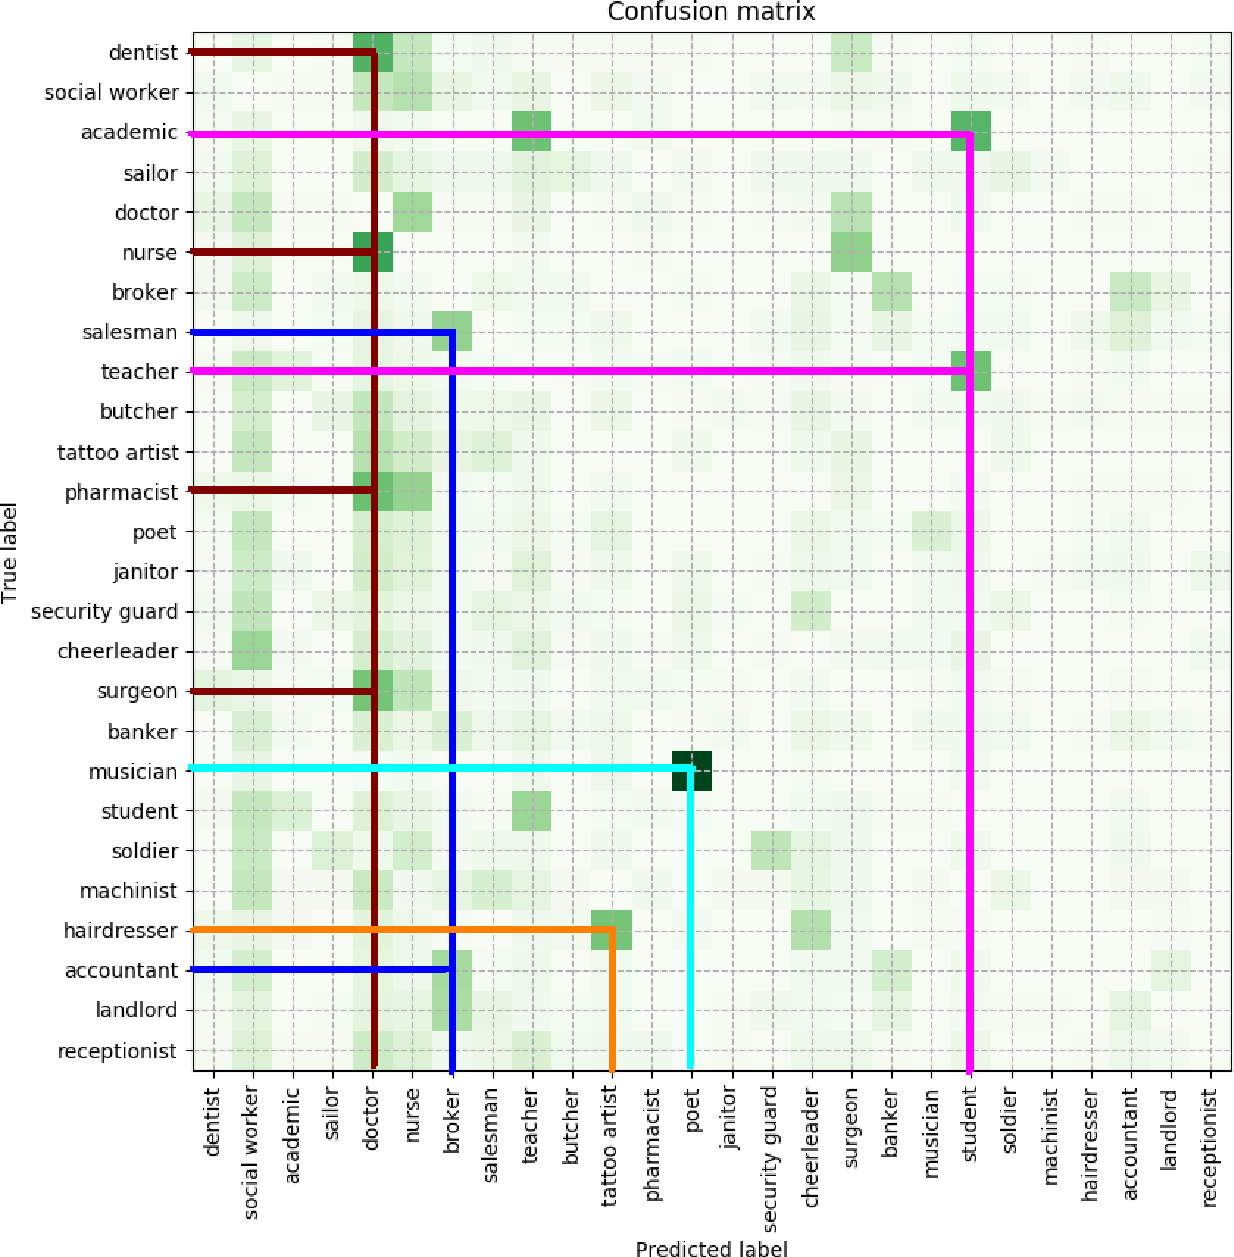
\includegraphics[scale=0.5]{imgs/profession_confusion.pdf}
\vspace{0.3cm}
\caption{Confusion matrix for \emph{profession}  with \charm{KNRM} on \emph{unseen} experiments, with some values removed for brevity. Unseen values are aggregated across folds. 
Darker cells indicate more misclassifications. The lines illustrate misclassifications of interest.
}
   \label{conf_prof}
\end{figure}

%\begin{figure*}[h!]
% \centering
% \begin{subfigure}{.49\textwidth}
%   \centering
%   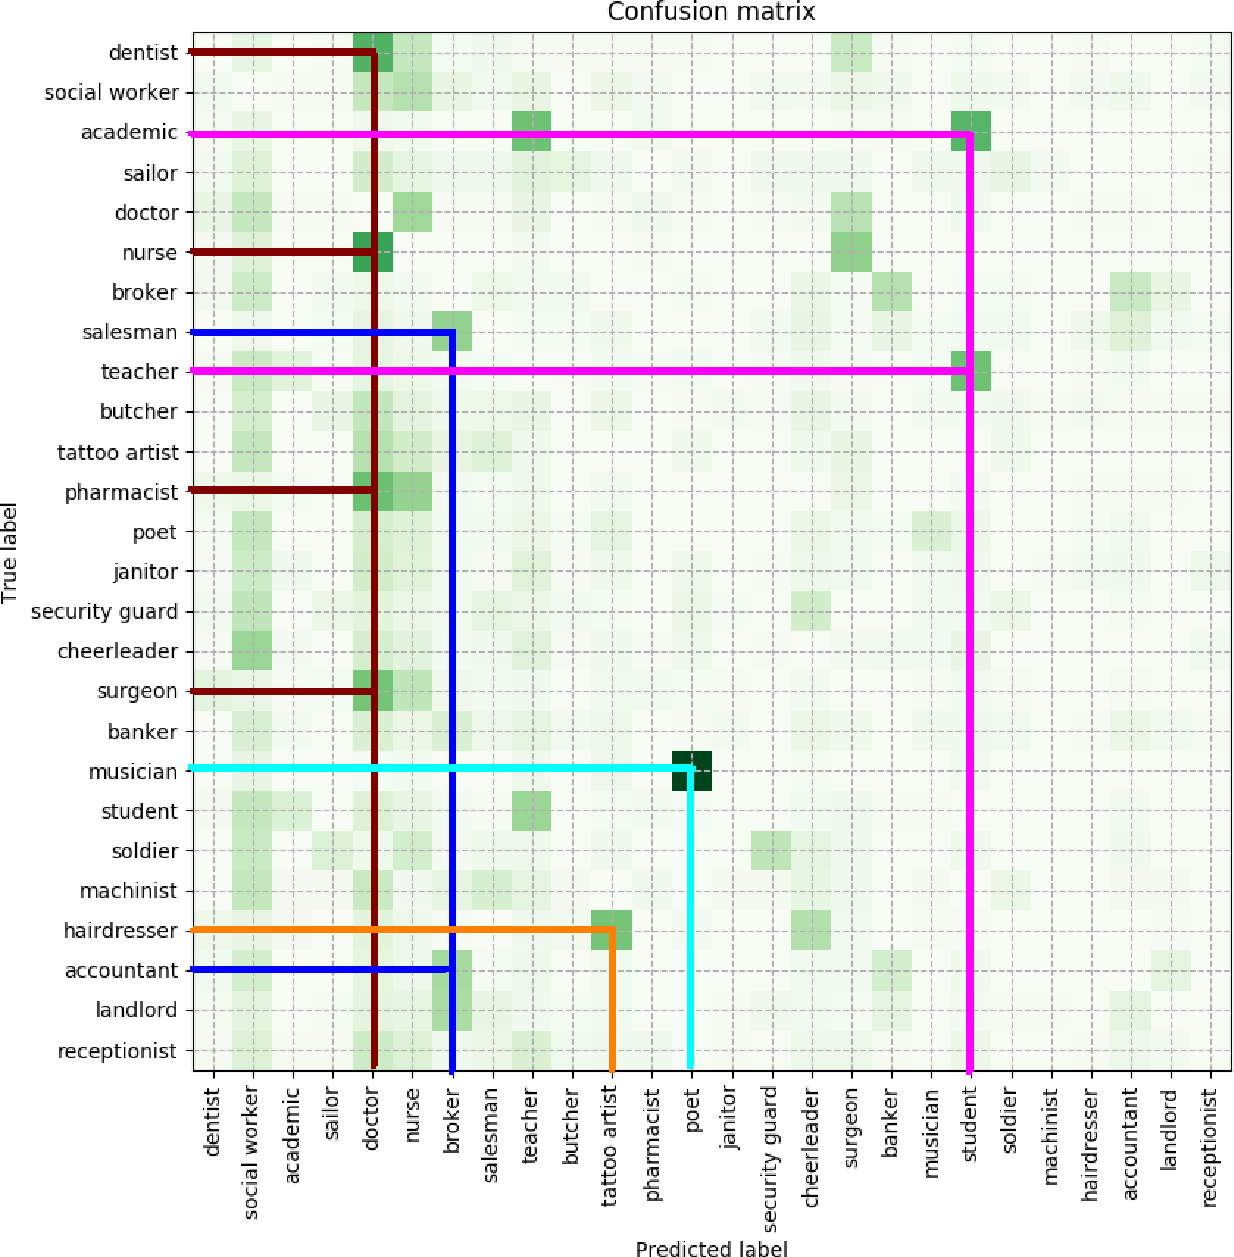
\includegraphics[scale=0.32]{imgs/profession_confusion.pdf}
%   \caption{\textit{profession}}
%   \label{conf_prof}
% \end{subfigure}
% \begin{subfigure}{.49\textwidth}
%   \centering
%   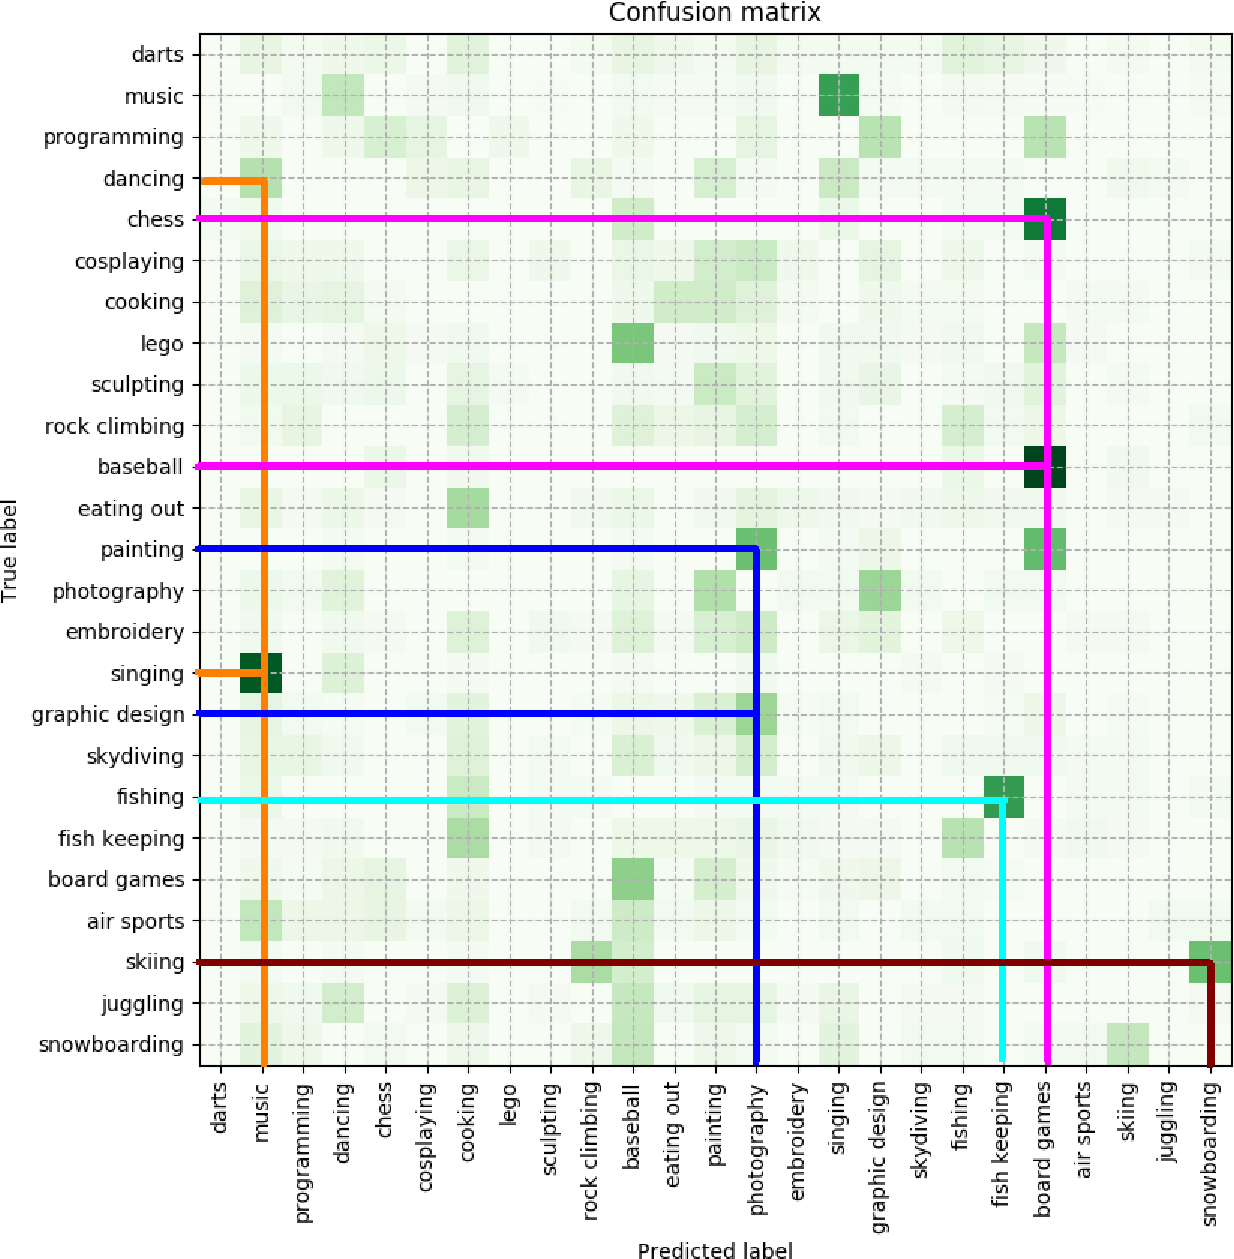
\includegraphics[scale=0.32]{imgs/hobby_confusion.pdf}
%   \caption{\textit{hobby}}
%   \label{conf_hob}
% \end{subfigure}
%\vspace*{-0.3cm}
%\caption{Confusion matrix for \emph{profession} and \emph{hobby} with \charm{KNRM} on \emph{unseen} experiments, with some values removed for brevity. Unseen values are aggregated across folds. 
%Darker cells indicate more misclassifications. The lines illustrate misclassifications of interest.
%}
%\label{fig:conf-profession-hobby}
%\end{figure*}


\paragraphHd{Analysis of top ranked documents}
For each attribute value, we collected all documents that were returned for a user with the given value as the ground-truth label. We then averaged the scores for each document and selected the top 5 retrieved documents from \wiki{category},
shown in Table \ref{tab:top_pages} for several \emph{profession} and \emph{hobby} attribute values.

It is interesting to observe that in spite of the common lexicon for some similar values, the model manages to retrieve documents which are relevant to a particular value, e.g., documents for \textit{investor}  are distinct from other financial-related professions, like \textit{broker} or \textit{salesman}.
It is also worth mentioning that the retrieved pages for \textit{investor} and \textit{ice hockey} are rather the pages for related lexicon (e.g., `\textit{venture capital}' and `\textit{playoff beard}' respectively), which shows the ability of CHARM to detect indirect cues.


\begin{table*}[t!] \sffamily
    \centering
    \footnotesize
    \begin{adjustbox}{width=0.98\textwidth}
    \begin{tabular}{llll}
\toprule
                            \multicolumn{2}{c}{\attribute{profession}} & \multicolumn{2}{c}{\attribute{hobby}}                                                                                                                 \\
\cmidrule(lr){1-2} \cmidrule(lr){3-4}
                            \textbf{firefighter} (MRR=0.46)                & \textbf{investor} (MRR=0.52)                      & \textbf{knitting} (MRR=0.68)                                                & \textbf{ice hockey} (MRR=0.68)                         \\ \midrule
                            Firefighter                                          & Index\_fund                                       & Yarn\_over                                               & Extra\_attacker                                     \\
                            Firefighter\_assist\_and\_search\_team              & Venture\_capital                                  & Brioche\_knitting                                        & Ice\_hockey\_rules                                  \\
                            Calvert\_County\_Fire-Rescue-EMS                    & Treasury\_management                              & Combined\_knitting                                       & Neutral\_zone\_trap                                 \\
                            Firefighter\_arson                                  & Buy\_side                                         & Flat\_knitting                                          & Playoff\_beard                                      \\
                            Fire\_captain                                       & Sovereign\_wealth\_fund                           & Tunisian\_crochet                                        & Line\_(ice\_hockey)                                 \\  \bottomrule
\end{tabular}
    \end{adjustbox}
    \caption{\charm{KNRM}'s top 5 retrieved documents per attribute value.}
    \label{tab:top_pages}
\end{table*}

\section{CHARM Demo}

In this section we present a web demonstration platform, accessible at \url{https://d5demos.mpi-inf.mpg.de/charm}, that showcases CHARM as a predictive model for extracting personal knowledge from conversational utterances \cite{tigunova2021exploring}. The contribution of such system is twofold. First, the demonstration can help users protect their privacy by identifying parts of their generated content that could give away personal information. Second, the system shows in detail how the model arrives at the prediction, which is rarely 
reflected in most automated extraction systems for personal facts.

\subsection{Motivation} 

Personal knowledge is a versatile resource that is valuable for a wide range of downstream applications. As observed in Chapter \ref{chap_backgr}, there has been ample research on automatically extracting or inferring personal knowledge. The developed models for conversational data predict a wide range of personal attributes from basic demographics and personality features to fine-grained interests and biography facts.

Such models can benefit many practical applications, yet they potentially endanger privacy. Thus, users should be given an opportunity to assess how the extraction models work in a transparent way. First, this enables users to explore how much personal information can be revealed from what they say online. Second, this helps to explain the reasoning leading to specific personalized ads and recommendations.

To address this issue we develop a demonstration platform for personal knowledge extraction methods, with CHARM as the underlying model. Such setting gives users a chance to directly observe the model's predictions (as opposed to, for example, trying to interpret the recommendations and ads on the websites).

We demonstrate CHARM's predictive capacity in two possible scenarios. The first setting demonstrates how a chatbot can interact with users to collect personal facts, designed as a guessing game. 
This provides the users with an opportunity to give creative answers and explore the model's capabilities, particularly in inferring the attribute values from given \emph{cues} (e.g., `\textit{pool}', `\textit{paddles}') instead of explicit \emph{mentions} (e.g., `\textit{swimming}'). 
Users can also try out some rare values (e.g., \emph{quilting}) or test how fine-grained the predictions can be (e.g., \emph{curling} instead of \emph{sports}). 
The second scenario involves applying CHARM on the real users' posts on social media. 

The proposed CHARM demonstration enables the users to \emph{(i)} see what personal information is disclosed by their answers or social media posts, and \emph{(ii)} get explanations on how the prediction was made. This supports users' privacy and model's transparency, which are rarely considered by personalized downstream applications, such as search or recommendation engines.

%The top scoring attribute values are yielded by the model as predictions.
%Explanations are given in the form of textual cues found in the input utterances, as well as retrieved web documents used to indicate the attribute values. The users can then identify revealing utterances and see how the predictions change if they modify the lexicon they use. 
%Moreover, we provide an \emph{unseen} mode  to examine how robust the model is for the values that were not seen during training.

\subsection{Demonstration platform}

\label{sec:demo}

Our demonstration system supports prediction of two personal attributes: \textit{profession} and \textit{hobby}, and incorporates two input scenarios: \emph{chatbot} and \emph{social media} settings.

\subsubsection{Input scenarios}

\paragraph{Chatbot setting.} Personal assistants enhanced with background knowledge about their users can give better responses and initiate more interesting conversations.
In this setting, we imitate how an intelligent assistant can infer personal facts from interactions with its user without asking explicit questions, such as \emph{``What is your job?''}. 
The interaction is designed as a game, where the chatbot asks several attribute-related questions, as shown in Figure~\ref{conv}.

\begin{figure}[th!]
\centering
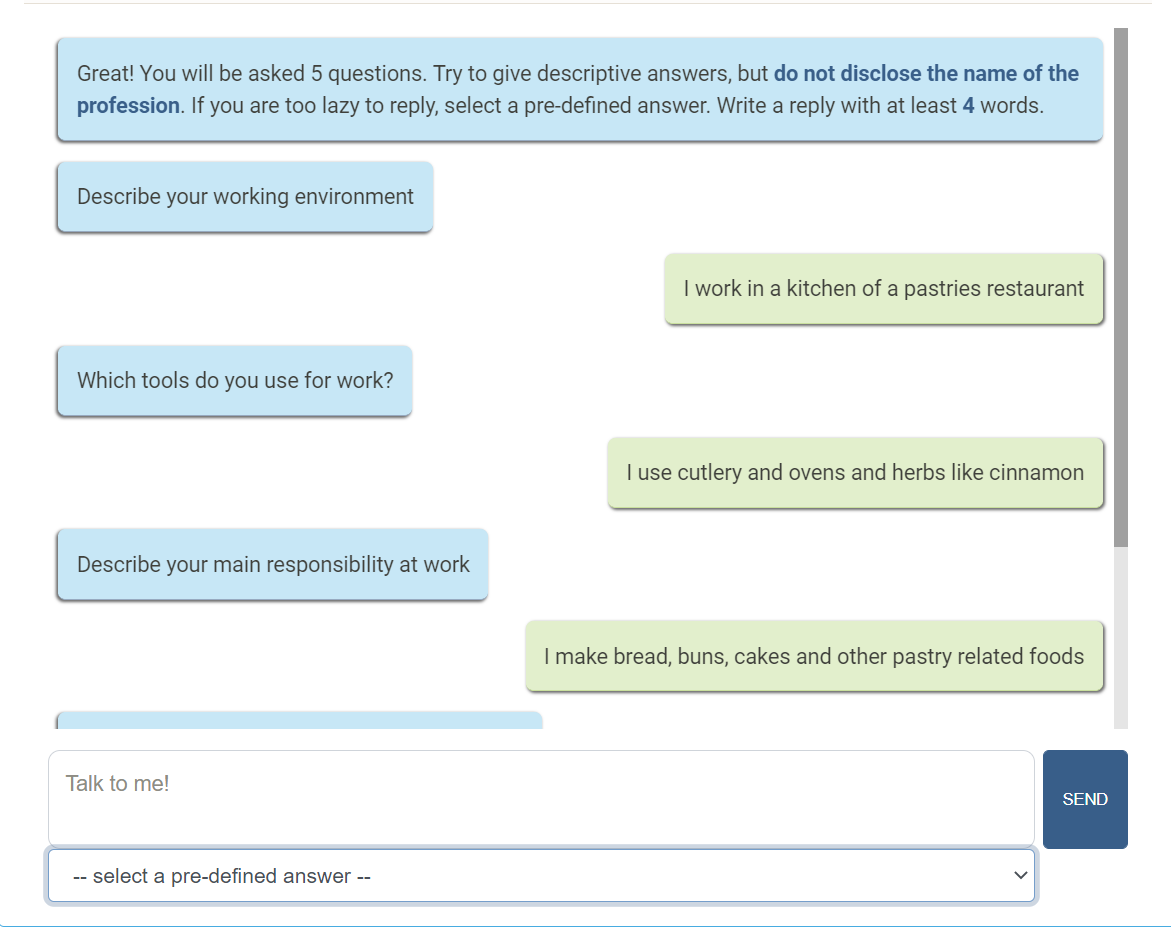
\includegraphics[width=0.85\textwidth]{imgs/conv-baker.png}
\vspace*{-0.3cm}
\caption{Chatbot conversation.}
\label{conv}
\end{figure}

Users are supposed to avoid mentioning the attribute value they have in mind, but rather to provide the chatbot with indirect cues like \emph{``I work in a \textbf{kitchen}''} for the \emph{``Describe your working environment''} question. The number of questions is fixed to 5, which should provide enough cues in the user's utterances to predict the correct attribute value without a lengthy interaction. We also require that the user's response to a question contains at least four words. 

To give users an idea of how responses should look, we provide a sample reply to each question, which the user can choose instead of typing their own responses. Each reply is designed as if it was given by a person with some pre-defined attribute value. For example, for the chat-bot request \textit{``Describe the place where you do your hobby''}, we add a predefined reply \textit{``It is a pool or open water''} related to \textit{hobby:swimming}. 

\paragraph{Social media setting.} 
Social media traces of online users are utilized by large companies for personalizing their services and ads, making them more interesting and relevant. However, the users have neither control nor understanding of how their personal information was inferred and which parts of their content revealed it. Ideally, the users should be given an opportunity to identify and exclude their posts which can potentially expose personal facts. 

In the social media scenario, we show how CHARM 
can dig through the vast amount of 
noisy 
conversational data in social media to find accurate cues for prediction.
Users can type or paste their social media posts (e.g., Reddit submissions) into the social media interface of our demonstration platform. Together with CHARM's predictions, the users will be provided with the information which parts of their utterances were used by the predictive model. It provides an opportunity to delete or modify the exposing content, and to check whether the model can still arrive at the same prediction after a partial content removal.

As in the chatbot scenario, we provide samples of synthetic user-generated content, resembling submissions in Reddit discussion threads, corresponding to pre-defined attribute values.
%that are often noisy, colloquial and unstructured.


\begin{figure}[th!]
    \centering
    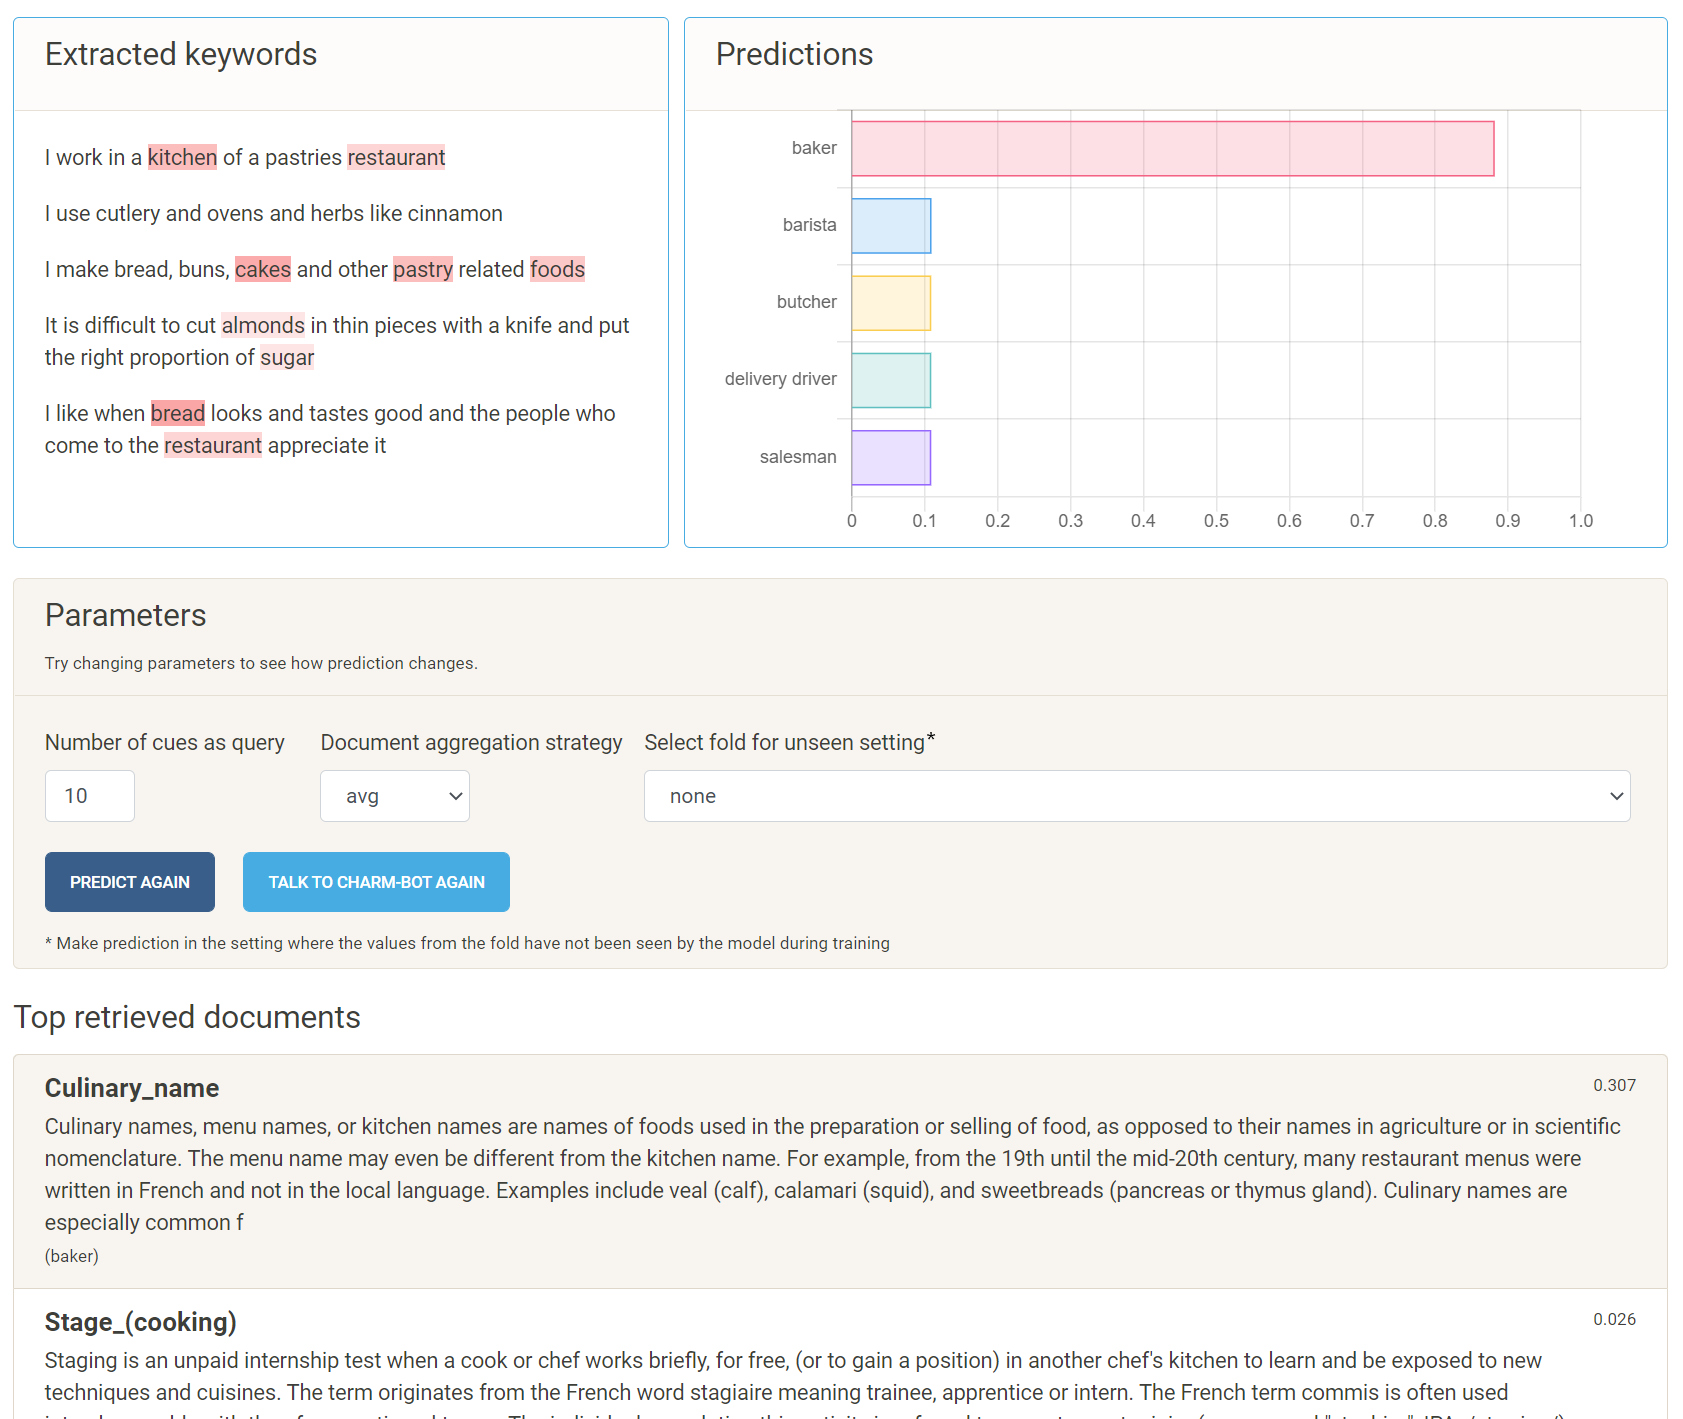
\includegraphics[width=0.95\textwidth]{imgs/prediction-baker.png}
    \caption{CHARM prediction result.}
    \label{pred_img}
\end{figure}

\subsubsection{Prediction results} 
As shown in Figure \ref{pred_img}, the prediction page presented to the user consists of intermediate results for both components of CHARM (\textit{term scoring model} and \textit{document ranker}) and the final prediction. To show the keyword selection step, we highlight the words in the user's utterances with an intensity that corresponds to the words' scores given by the {term scoring model}. The results for the document ranking step are presented as a sorted list of 10 top scoring documents. Each document is linked to the original article on the web. Finally, we show top 5 attribute value predictions after aggregating document scores. We normalized them to $[0,1]$ scale for interpretability when comparing the model's confidence in predicting each value. 

\subsubsection{Model parameters} 
The demonstration allows the users to explore how CHARM's predictions change depending on its two hyperparameters: the \emph{number of extracted keywords} and the \emph{document aggregation strategy}. 
We set the default number of extracted keywords as $\frac{1}{3}$ of the number of meaningful terms in the input utterances (after removing stopwords and digits), 
with 10 as the maximum value.
Setting the number of keywords too high can result in a noisy query and inadequate behaviour of the retrieval model. 
On the other hand, small number of keywords can be insufficient for accurate document retrieval.

As the document aggregation strategy, the user can choose between \texttt{max} and \texttt{average} functions. \texttt{Max} operation is useful when the document collection is noisy and the prediction score should come from a single most relevant document per attribute value. The \texttt{average} function is good to provide a balanced prediction based on all available documents, protecting the result from being spoilt by an inappropriate top scoring document. For this reason we selected \texttt{average} as the default aggregation function.

We selected to use \charm{KNRM} as the underlying model and \wiki{category} as document collection for our demonstration platform. As shown in the experiments described in Section \ref{charm_results}, this combination of ranker and document collection shows superior performance in most test cases. \wiki{category} is a sweet spot between simple \wiki{page}, which can only provide trivial explanations with pages matching attribute value name, and Web-search collection, which is difficult for the end-user to interpret because of noisy and ill-formatted pages. %On the other hand, \wiki{category} shows how CHARM's predictions can be determined by the topical pages from the same category.
 
\subsubsection{Unseen scenario} 
We also showcase CHARM's ability to predict attribute values
that are lacking training samples.
We train 10 variants of the model, in which each model has seen samples from only 90\% of the attribute values during training; 10\% of the attribute values are \emph{unseen}. 
In our web interface, the users can try to make a prediction using one of those models
by selecting the option where the listed attribute values are unseen. 
For example, for the input utterances \{\emph{``I was pedaling the whole evening''}, \emph{``I don't like long walks, I like spending time on my bike''}\}, it can be interesting to see the prediction result by the model not trained on hobby value \emph{cycling}. 

\subsection{Case study}
\label{sec:case-study}

In this section we present a walk-though scenario for the chatbot setting. As input we take a set of utterances from a pre-defined personality having \textit{profession}: \textit{baker}. In the first step, the chatbot asks the user 5 questions, such as \emph{``How do you start your day at work?''}. We give an excerpt of the conversation between the user and the chatbot in Figure \ref{conv}. 

On the next step the user is taken to the prediction result page, shown in Figure~\ref{pred_img}. Using the default heuristic, CHARM extracts \nolinebreak 9 keywords from the input.
The resulting query thus becomes \textit{``kitchen restaurant cakes pastry foods almonds sugar bread restaurant''}. From Figure \ref{pred_img} it can be seen that the words `\textit{cakes}', `\textit{bread}' and `\textit{pastry}' were assigned high scores by the term scoring model, whereas more general words, like `\textit{restaurant}', were included in the query but received lower scores.

The default document score aggregation strategy is \texttt{average}, which helps to overcome the influence of the top scoring document \emph{wiki:Stage\_(cooking)} (a culinary internship), which was automatically labeled as \textit{student}. 
Thus, if the user changes the aggregation function to \texttt{max}, the effect of document scoring makes \emph{baker} and \emph{student} almost equally probable. 

The qualitative results of varying the parameters of CHARM on our exemplary input are shown in Table \ref{param_change}. 
Setting the number of keywords to 2 still does not prevent CHARM from making a correct prediction using a concise query \textit{``bread ovens''}. However, the model is not robust with a long query, resulting in the ranker yielding many documents equally relevant to this query, like \emph{baker}, \emph{barista} and \emph{butcher} pages.

Finally, the user can inspect the behaviour of CHARM in the \emph{unseen} setup, when the value \emph{baker} was not present in the training data. To do that the user should select an unseen fold from the dropdown list, which contains the value \emph{baker}. As shown in Table \nolinebreak\ref{param_change}, CHARM is still capable of predicting the correct value. In contrast to the normal \textit{seen} setting, the difference in scores for correct and incorrect predictions is less.

\begin{table}[]
    \centering
\begin{adjustbox}{width=0.75\textwidth}
\begin{tabular}{ccc|cl}
\toprule
\begin{tabular}[c]{@{}c@{}}number of \\ keywords\end{tabular} & \begin{tabular}[c]{@{}c@{}}aggregation \\ strategy\end{tabular} & \begin{tabular}[c]{@{}c@{}}seen/unseen \\ setting\end{tabular} & \begin{tabular}[c]{@{}c@{}}correct \\ prediction score\end{tabular} & \begin{tabular}[c]{@{}c@{}}best incorrect \\ prediction score\end{tabular} \\ \midrule
10                                                            & avg                                                             & seen                                                           & 0.91                                                                & 0.19 (barista)                                                                      \\
\textbf{2}                                                    & avg                                                             & seen                                                           & 0.88                                                                & 0.19 (sailor)                                                                      \\
\textbf{25}                                                   & avg                                                             & seen                                                           & 0.85                                                                  & 0.85 (barista)                                                                      \\
10                                                            & \textbf{max}                                                    & seen                                                           & 0.89                                                                & 0.77 (student)                                                                       \\
10                                                            & avg                                                             & \textbf{unseen}                                                & 0.91                                                                & 0.32 (butcher) \\                      \bottomrule                                  
\end{tabular}
\end{adjustbox}
    \caption{Prediction scores based on CHARM parameters.}
    \label{param_change}
\end{table}

\section{Conclusion and Discussion}
\section{Conclusion}

We presented PRIDE, a model for inferring fine-grained relationships from conversations. To our best knowledge, PRIDE is the first model to predict \textit{directed, multilabel} speakers' relationships. PRIDE leverages the hierarchical dialogue structure to efficiently handle lengthy conversational history. The novelty of our architecture is the additional signals of speakers' demographics and speech style, which significantly improve relationship prediction.

PRIDE outperforms state-of-the-art baselines and demonstrates effective transfer learning on different types of dialogue data. %In ablation experiments we demonstrate that the proposed architecture improves the model's predictions. 
PRIDE is designed to perform inference on long conversational sequences; however, we experimentally show PRIDE's ability to make accurate predictions for shorter interactions too. 

To support future work on this topic, we created and released the largest labeled collection of relationships in conversations, which improves over existing datasets by including directed multilabel relationships.

\subsection{Discussion}

In this subsection we discuss several limitations of the current work and propose directions for further improvements of PRIDE:

\begin{itemize}
    \item \textbf{Leveraging other types of conversational data.} Inferring relationships in real-life user conversations is the use case motivating our research. Thus, we find it important to evaluate PRIDE's transfer learning capabilities to other conversational datasets to ensure that it can generalize. Our choice of the dataset was constrained by the complexity of labeling dialogues with relationship labels; we leave it for future work to obtain more diverse relationship datasets (for example, social media interactions or telephone transcripts).
    
    \item \textbf{Improving performance on directed relationships.} Predicting asymmetric relationships has been overlooked in the prior works; yet accurately distinguishing them is important for practical applications. For instance, an intelligent assistant can recommend completely different items, depending of whether the user is asking for a birthday present suggestions for her \textit{parent} or her \textit{child}. Thus, we find it necessary to further improve PRIDE's performance on asymmetric relationships.
    
    \item \textbf{Incorporating more personal attributes.} In our experiments we showed that prediction of interpersonal relationships can benefit from adding speakers' attributes. We find it interesting to experiment on adding other personal information, such as \textit{occupation} or \textit{ethnicity}.

    \item \textbf{Joint prediction of personal attributes and interpersonal relationships.} The current version of PRIDE supports incorporating precomputed ground truth information about the speakers' ages. In the scenario when personal attribute labels are not available, one option is to use a predictive model (such as HAM) to provide such information on the fly. Joint training of the relationship and speakers' attribute prediction models could improve their performance, as relationships and personal attributes are interdependent.

    \item \textbf{Considering multispeaker conversations.} The current dataset used in experiments with PRIDE was limited to uninterrupted dialogue spans between two characters. This limitation was due to the difficulty of distinguishing the addressee of an utterance when more than 2 speakers are present. In real life people often interact in a group, thus considering only speaker pairs will result in losing useful cues for predictions. Therefore, extension of the current model to handle multi-speaker conversations should be further investigated.
    %Therefore, we find it important to investigate the ways the current model can be extended to handle multi-speaker dialogues.

    
\end{itemize}

%The last research direction can also be generalized to the other models discussed in the current thesis. For instance, the people who communicate are often in the same age group and = have the same \textit{hobbies} (if they are friends) or \textit{professions} (if they are colleagues). We highlight simultaneous predictions of personal attributes and relationships using speaker network as a compelling future research direction.

\bibliographystyle{abbrvnat}
\bibliography{bibliography}

\end{document}
